\section{Generic compositions}

\begin{description}
  \item[Encrypt-and-MAC]
  \item[MAC-then-Encrypt]
  \item[Encrypt-then-MAC]
\end{description}

\begin{figure}
  \centering
  \begin{subfigure}[b]{0.3\textwidth}
    \centering
    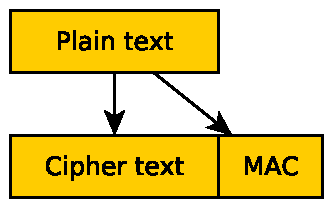
\includegraphics[width=0.9\textwidth]{images/encrypt-and-mac.pdf}
    \caption{Encrypt-and-MAC}
  \end{subfigure}
  \begin{subfigure}[b]{0.3\textwidth}
    \centering
    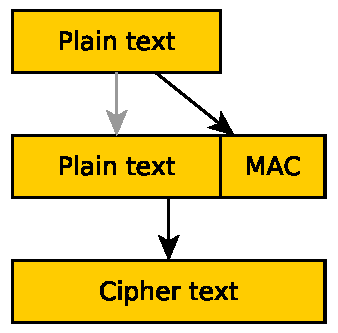
\includegraphics[width=0.9\textwidth]{images/mac-then-encrypt.pdf}
    \caption{MAC-then-encrypt}
  \end{subfigure}
  \begin{subfigure}[b]{0.3\textwidth}
    \centering
    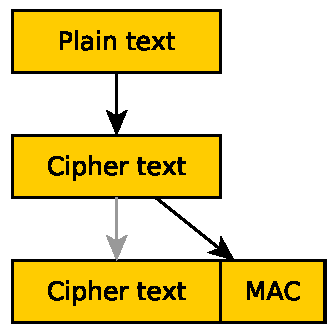
\includegraphics[width=0.9\textwidth]{images/encrypt-then-mac.pdf}
    \caption{Encrypt-then-MAC}
  \end{subfigure}
  \caption{Generic compositions of Authentized Encryption}
\end{figure}
